\documentclass[aspectratio=169]{beamer}
\usetheme{Madrid}
\usecolortheme{beaver}
\usepackage[utf8]{inputenc}
\usepackage[T1]{fontenc}
\usepackage{tikz}
\usepackage{amssymb}
\usepackage{graphicx}
\setbeamertemplate{navigation symbols}{}
\setbeamercolor{title}{fg=white,bg=cyan!60!black}
\setbeamercolor{frametitle}{fg=white,bg=cyan!50!black}
\setbeamercolor{block title}{bg=cyan!15,fg=black}
\setbeamercolor{block body}{bg=cyan!5,fg=black}

\title{G6 — Collision \& Physics}
\subtitle{Lesson 1: Hitbox Check}
\author{ByteForge --- Grade 7 --- Game Maker}
\date{}

\begin{document}

\begin{frame}
    \titlepage
\end{frame}

\begin{frame}{The distance formula — real Pythagoras}
    \Large
    \texttt{dist = sqrt((x2-x1)\textasciicircum{}2 + (y2-y1)\textasciicircum{}2)} — literally Pythagoras' theorem, applied to two circle centres.

    \begin{center}
    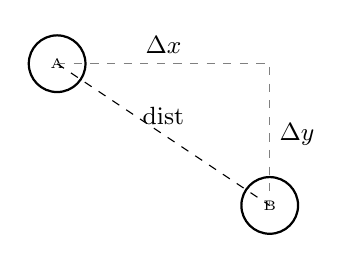
\begin{tikzpicture}[scale=0.9]

        \draw[thick] (0,0) circle (0.4);
        \node at (0,0) {\tiny A};
        \draw[thick] (3,-2) circle (0.4);
        \node at (3,-2) {\tiny B};
        \draw[dashed] (0,0) -- (3,-2) node[midway, above] {\small dist};
        \draw[dashed, gray] (0,0) -- (3,0) -- (3,-2);
        \node[above] at (1.5,0) {\small $\Delta x$};
        \node[right] at (3,-1) {\small $\Delta y$};
    \end{tikzpicture}
    \end{center}
\end{frame}

\begin{frame}{Your Turn}
    \Large
    Open the student map, find \textbf{G6 — Collision \& Physics}, and complete
    the \textbf{Hitbox Check} challenge --- everything you just saw, they now do themselves.
\end{frame}

\end{document}
